%%%%%%
%
% PROJECT 13 - Numerical/Euler/Runge-Kutta
%
% filename: numerical.tex
% last modified: 2015-3-15
%


\documentclass
[justified,nohyper]
{tufte-handout}

\usepackage{amsmath}
\usepackage{tabularx}

\usepackage{booktabs}
\usepackage{graphicx}
\usepackage{kmath,kerkis} % The order of the packages matters; kmath changes the default text font
\usepackage[T1]{fontenc}

\begin{document}
\section{Advanced Calculus Project 13: Three Famous Numbers}

\newthought{In this project,} you will learn how to approximate three famous
numbers using differential equations. The three famous numbers are $e$,
$\pi$, and $\ln 2$. To find approximations to these three numbers, you will
program SAGE to estimate solutions to a differential equation using two different
methods. The first method, Euler's method, you already know. The second method,
Runge-Kutta, will require a little bit of research.

Let's start with the differential equation we will use to find the number $e$.
\[
	\dfrac{dy}{dx} = y \hspace{0.5cm} \text{,} \; y(0)=1
\]
The solution to this differential equation is $y=e^{x}$, so if we can approximate
$y(1)$ we have found an approximation to $e$.

\section*{Euler's Method}
Your task is to use Euler's method in a loop to approximate $y(1)$ with four
different step sizes: 1, 2, 20, 50, 100, 1000. Plot the slope field for the differential
equation, along with line segments and points for the four different
approxmations. Your graph should look something like this:

\begin{center}{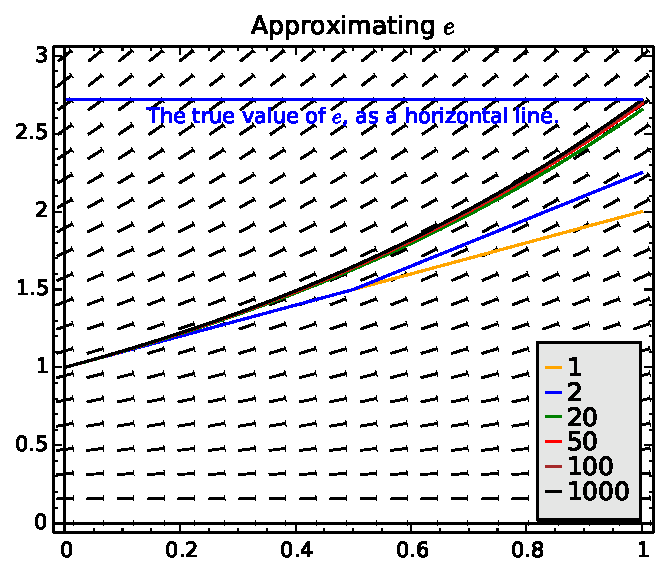
\includegraphics[width=8cm]{eulers.pdf}}\end{center}

Along with the graph, you should print out a table showing the results of your
calculations.

\begin{center}
\begin{tabularx}{\textwidth}{|p{3cm} |p{3cm} |p{3.65cm}|}
	\hline
	Number of Steps & $y(1)$ & Error \\
	\hline
	1 & $(1,2.00000000)$ & 0.71828182 \\
	\hline
	2 & $(1,2.25000000)$ & 0.46828182 \\
	\hline
	20 & $(1,2.65329770)$ & 0.06498412 \\
	\hline
	50 & $(1,2.69158802)$ & 0.02669379 \\
	\hline
	100 & $(1,2.70481382)$ & 0.01346799 \\
	\hline
	1000 & $(1,2.71692393)$ & 0.00135789 \\
	\hline
\end{tabularx}
\end{center}

Repeat this process for the other two numbers using the same step sizes that
were specified above: 1, 2, 20, 50, 100, 1000. Here are the differential
equations that you will need to use.

For $\pi$:
\[
	\dfrac{dy}{dx} = \dfrac{4}{1+x^2} \hspace{0.5cm} \text{,} \; y(0)=0
\]

For $\ln 2$:
\[
	\dfrac{dy}{dx} = \dfrac{1}{x} \hspace{0.5cm} \text{,} \; y(1)=0
\]

For each of the two differential equations, solve them analytically to show
that the resulting approximation is correct.

\section*{Runge-Kutta}
Euler's method is nice. The algorithm takes an initial point on the solution
graph and uses the slope and step size to compute an approximation to another
point on the solution graph.
The basic idea is that the smaller the step size, the more
accurate the approximation.

Runge-Kutta methods simply use more information to compute the next approximation.
The basic idea is the same. Start with a known point on the solution curve and use
information about the differential equation to compute an approximation to
another point on the solution graph.

The difference with Runge-Kutta is that it is computationally less expensive.
In other words, we can get a good approximation without increasing the step size.
The less steps we have to take, the better.

You task will be to research Runge-Kutta methods for solving differential equations,
and program SAGE to compute approximations to the three famous numbers. Use
the same differential equations and initial conditions, as well as the same
step sizes. Compare your results and comment on the accuracy.

The wikipedia article on Runge-Kutta is a great place to start. Your final paper
should include some basic outline of Runge-Kutta methods and how they work. This
doesn't have to be in great detail, but should provide the reader with enough
background that they feel confident in the solution methodology.

\section*{Your Report}
At a minimum, your report must contain approximations of the three famous numbers
using both Euler's method and Runge-Kutta methods with step sizes as given
in this project description. For each approximation, there
should be a table of numbers and a graph showing each approximation along with
a slope field for that differential equation, as well as the exact value of
the number you are approximating. Six tables and six graphs along with some
text describing what you did. You do not need to include the code used from SAGE
in your report, although you may do so if you wish.

\end{document}